%  LaTeX support: latex@mdpi.com 
%  For support, please attach all files needed for compiling as well as the log file, and specify your operating system, LaTeX version, and LaTeX editor.

%=================================================================
\documentclass[journal,article,submit,moreauthors,pdftex]{Definitions/mdpi} 

% For posting an early version of this manuscript as a preprint, you may use "preprints" as the journal and change "submit" to "accept". The document class line would be, e.g., \documentclass[preprints,article,accept,moreauthors,pdftex]{mdpi}. This is especially recommended for submission to arXiv, where line numbers should be removed before posting. For preprints.org, the editorial staff will make this change immediately prior to posting.

%--------------------
% Class Options:
%--------------------
%----------
% journal
%----------
% Choose between the following MDPI journals:
% acoustics, actuators, addictions, admsci, adolescents, aerospace, agriculture, agriengineering, agronomy, ai, algorithms, allergies, analytica, animals, antibiotics, antibodies, antioxidants, appliedchem, applmech, applmicrobiol, applnano, applsci, arts, asi, atmosphere, atoms, audiolres, automation, axioms, batteries, bdcc, behavsci, beverages, biochem, bioengineering, biologics, biology, biomechanics, biomedicines, biomedinformatics, biomimetics, biomolecules, biophysica, biosensors, biotech, birds, bloods, brainsci, buildings, businesses, cancers, carbon, cardiogenetics, catalysts, cells, ceramics, challenges, chemengineering, chemistry, chemosensors, chemproc, children, civileng, cleantechnol, climate, clinpract, clockssleep, cmd, coatings, colloids, compounds, computation, computers, condensedmatter, conservation, constrmater, cosmetics, crops, cryptography, crystals, curroncol, cyber, dairy, data, dentistry, dermato, dermatopathology, designs, diabetology, diagnostics, digital, disabilities, diseases, diversity, dna, drones, dynamics, earth, ebj, ecologies, econometrics, economies, education, ejihpe, electricity, electrochem, electronicmat, electronics, encyclopedia, endocrines, energies, eng, engproc, entropy, environments, environsciproc, epidemiologia, epigenomes, fermentation, fibers, fire, fishes, fluids, foods, forecasting, forensicsci, forests, fractalfract, fuels, futureinternet, futuretransp, futurepharmacol, futurephys, galaxies, games, gases, gastroent, gastrointestdisord, gels, genealogy, genes, geographies, geohazards, geomatics, geosciences, geotechnics, geriatrics, hazardousmatters, healthcare, hearts, hemato, heritage, highthroughput, histories, horticulturae, humanities, hydrogen, hydrology, hygiene, idr, ijerph, ijfs, ijgi, ijms, ijns, ijtm, ijtpp, immuno, informatics, information, infrastructures, inorganics, insects, instruments, inventions, iot, j, jcdd, jcm, jcp, jcs, jdb, jfb, jfmk, jimaging, jintelligence, jlpea, jmmp, jmp, jmse, jne, jnt, jof, joitmc, jor, journalmedia, jox, jpm, jrfm, jsan, jtaer, jzbg, kidney, land, languages, laws, life, liquids, literature, livers, logistics, lubricants, machines, macromol, magnetism, magnetochemistry, make, marinedrugs, materials, materproc, mathematics, mca, measurements, medicina, medicines, medsci, membranes, metabolites, metals, metrology, micro, microarrays, microbiolres, micromachines, microorganisms, minerals, mining, modelling, molbank, molecules, mps, mti, nanoenergyadv, nanomanufacturing, nanomaterials, ncrna, network, neuroglia, neurolint, neurosci, nitrogen, notspecified, nri, nursrep, nutrients, obesities, oceans, ohbm, onco, oncopathology, optics, oral, organics, osteology, oxygen, parasites, parasitologia, particles, pathogens, pathophysiology, pediatrrep, pharmaceuticals, pharmaceutics, pharmacy, philosophies, photochem, photonics, physchem, physics, physiolsci, plants, plasma, pollutants, polymers, polysaccharides, proceedings, processes, prosthesis, proteomes, psych, psychiatryint, publications, quantumrep, quaternary, qubs, radiation, reactions, recycling, regeneration, religions, remotesensing, reports, reprodmed, resources, risks, robotics, safety, sci, scipharm, sensors, separations, sexes, signals, sinusitis, smartcities, sna, societies, socsci, soilsystems, solids, sports, standards, stats, stresses, surfaces, surgeries, suschem, sustainability, symmetry, systems, taxonomy, technologies, telecom, textiles, thermo, tourismhosp, toxics, toxins, transplantology, traumas, tropicalmed, universe, urbansci, uro, vaccines, vehicles, vetsci, vibration, viruses, vision, water, wevj, women, world 

%---------
% article
%---------
% The default type of manuscript is "article", but can be replaced by: 
% abstract, addendum, article, book, bookreview, briefreport, casereport, comment, commentary, communication, conferenceproceedings, correction, conferencereport, entry, expressionofconcern, extendedabstract, datadescriptor, editorial, essay, erratum, hypothesis, interestingimage, obituary, opinion, projectreport, reply, retraction, review, perspective, protocol, shortnote, studyprotocol, systematicreview, supfile, technicalnote, viewpoint, guidelines, registeredreport, tutorial
% supfile = supplementary materials

%----------
% submit
%----------
% The class option "submit" will be changed to "accept" by the Editorial Office when the paper is accepted. This will only make changes to the frontpage (e.g., the logo of the journal will get visible), the headings, and the copyright information. Also, line numbering will be removed. Journal info and pagination for accepted papers will also be assigned by the Editorial Office.

%------------------
% moreauthors
%------------------
% If there is only one author the class option oneauthor should be used. Otherwise use the class option moreauthors.

%---------
% pdftex
%---------
% The option pdftex is for use with pdfLaTeX. If eps figures are used, remove the option pdftex and use LaTeX and dvi2pdf.

%=================================================================
% MDPI internal commands
\firstpage{1} 
\makeatletter 
\setcounter{page}{\@firstpage} 
\makeatother
\pubvolume{1}
\issuenum{1}
\articlenumber{0}
\pubyear{2021}
\copyrightyear{2020}
%\externaleditor{Academic Editor: Firstname Lastname} % For journal Automation, please change Academic Editor to "Communicated by"
\datereceived{} 
\dateaccepted{} 
\datepublished{} 
\hreflink{https://doi.org/} % If needed use \linebreak
%------------------------------------------------------------------
% The following line should be uncommented if the LaTeX file is uploaded to arXiv.org
%\pdfoutput=1

%=================================================================
% Add packages and commands here. The following packages are loaded in our class file: fontenc, inputenc, calc, indentfirst, fancyhdr, graphicx, epstopdf, lastpage, ifthen, lineno, float, amsmath, setspace, enumitem, mathpazo, booktabs, titlesec, etoolbox, tabto, xcolor, soul, multirow, microtype, tikz, totcount, changepage, paracol, attrib, upgreek, cleveref, amsthm, hyphenat, natbib, hyperref, footmisc, url, geometry, newfloat, caption
\usepackage{cleveref}
\usepackage{overpic}
%=================================================================
%% Please use the following mathematics environments: Theorem, Lemma, Corollary, Proposition, Characterization, Property, Problem, Example, ExamplesandDefinitions, Hypothesis, Remark, Definition, Notation, Assumption
%% For proofs, please use the proof environment (the amsthm package is loaded by the MDPI class).

%=================================================================
% Full title of the paper (Capitalized)
\Title{Packet Optical Transport Network Slicing with Hard and Soft Isolation}

% MDPI internal command: Title for citation in the left column
\TitleCitation{Packet Optical Transport Network Slicing with Hard and Soft Isolation}

% Author Orchid ID: enter ID or remove command
\newcommand{\orcidauthorA}{0000-0000-0000-000X} % Add \orcidA{} behind the author's name
%\newcommand{\orcidauthorB}{0000-0000-0000-000X} % Add \orcidB{} behind the author's name

% Authors, for the paper (add full first names)
\Author{S.~Barguil$^1$, V.~López$^2$, L.M.~Contreras$^2$, O. González de Dios$^2$, A.~Alcalá$^1$, C.~Manso$^3$, P.~Alemany$^3$, R.~Casellas$^3$, R.~Martínez$^3$, D.~González-Pérez$^4$, X. Liu$^4$, J.M.~Pulido$^4$, J.P. Fernández-Palacios$^2$, R.~Muñoz$^3$, R.~Vilalta$^3$}

% MDPI internal command: Authors, for metadata in PDF
\AuthorNames{Firstname Lastname, Firstname Lastname and Firstname Lastname}

% MDPI internal command: Authors, for citation in the left column
\AuthorCitation{Barguil, S. et. al.}
% If this is a Chicago style journal: Lastname, Firstname, Firstname Lastname, and Firstname Lastname.

% Affiliations / Addresses (Add [1] after \address if there is only one affiliation.)
\address{%
$^{1}$ \quad Universidad Autónoma de Madrid, Madrid, Spain\\
$^{2}$ \quad Telefónica I+D, Madrid, Spain\\
$^{3}$ \quad Centre Tecnològic de Telecomunicacions de Catalunya (CTTC/CERCA), Castelldefels (Barcelona), Spain\\
$^{4}$ \quad Volta Networks, Barcelona, Spain}

% Contact information of the corresponding author
\corres{Correspondence: samier.barguil@estudiante.uam.es)}

% Current address and/or shared authorship
\firstnote{Current address: samier.barguil@estudiante.uam.es} 
%\secondnote{These authors contributed equally to this work.}
% The commands \thirdnote{} till \eighthnote{} are available for further notes

%\simplesumm{} % Simple summary

%\conference{} % An extended version of a conference paper

% Abstract (Do not insert blank lines, i.e. \\) 
\abstract{(Victor) We validate the deployment of isolated transport network slices in IP over DWDM network. To this end, an isolated transport network slice is deployed using multi-layer isolation mechanisms based on OpenConfig and ONF Transport API.
\\A single paragraph of about 200 words maximum. For research articles, abstracts should give a pertinent overview of the work. We strongly encourage authors to use the following style of structured abstracts, but without headings: (1) Background: place the question addressed in a broad context and highlight the purpose of the study; (2) Methods: describe briefly the main methods or treatments applied; (3) Results: summarize the article's main findings; (4) Conclusion: indicate the main conclusions or interpretations. The abstract should be an objective representation of the article, it must not contain results which are not presented and substantiated in the main text and should not exaggerate the main conclusions.}

% Keywords
\keyword{keyword 1; keyword 2; keyword 3 (List three to ten pertinent keywords specific to the article; yet reasonably common within the subject discipline.)} 

% The fields PACS, MSC, and JEL may be left empty or commented out if not applicable
%\PACS{J0101}
%\MSC{}
%\JEL{}

%%%%%%%%%%%%%%%%%%%%%%%%%%%%%%%%%%%%%%%%%%
% Only for the journal Diversity
%\LSID{\url{http://}}

%%%%%%%%%%%%%%%%%%%%%%%%%%%%%%%%%%%%%%%%%%
% Only for the journal Applied Sciences:
%\featuredapplication{Authors are encouraged to provide a concise description of the specific application or a potential application of the work. This section is not mandatory.}
%%%%%%%%%%%%%%%%%%%%%%%%%%%%%%%%%%%%%%%%%%

%%%%%%%%%%%%%%%%%%%%%%%%%%%%%%%%%%%%%%%%%%
% Only for the journal Data:
%\dataset{DOI number or link to the deposited data set in cases where the data set is published or set to be published separately. If the data set is submitted and will be published as a supplement to this paper in the journal Data, this field will be filled by the editors of the journal. In this case, please make sure to submit the data set as a supplement when entering your manuscript into our manuscript editorial system.}

%\datasetlicense{license under which the data set is made available (CC0, CC-BY, CC-BY-SA, CC-BY-NC, etc.)}

%%%%%%%%%%%%%%%%%%%%%%%%%%%%%%%%%%%%%%%%%%
% Only for the journal Toxins
%\keycontribution{The breakthroughs or highlights of the manuscript. Authors can write one or two sentences to describe the most important part of the paper.}

%%%%%%%%%%%%%%%%%%%%%%%%%%%%%%%%%%%%%%%%%%
% Only for the journal Encyclopedia
%\encyclopediadef{Instead of the abstract}
%\entrylink{The Link to this entry published on the encyclopedia platform.}
%%%%%%%%%%%%%%%%%%%%%%%%%%%%%%%%%%%%%%%%%%

\begin{document}
%%%%%%%%%%%%%%%%%%%%%%%%%%%%%%%%%%%%%%%%%%

\section{Introduction - Luis}

%The provisioning of connectivity services that guarantee a specific set of Service Level Objectives (SLO) regarding network resources is expected to benefit many use cases, such as beyond 5G networks or NFV and data center interconnects. Transport network slices provide connectivity coupled with a set of specific network resources commitment between several endpoints over a shared network infrastructure \cite{transportslice21}.  

%Each slice is associated with a tenant. Each tenant can control and manage all its slices. As underlying resource multi-tenancy is supported, multiple isolation options are provided, such as soft slicing and hard slicing. Soft network slicing focuses on QoS mechanisms that provide a dynamic allocation of available network resources to different traffic classes. An example of a soft network slice is a VLAN assigned to a customer to carry voice/data traffic, usually transported by LxVPNs. On the other hand, hard network slicing provides component virtualization and replication. An example of a hard network slice is routers (physical or virtual) under the same administrative domain, where services are configured between routers.

%The virtualization of the transport network can be exploited at the time of provisioning and orchestrating the virtualized service functions of the slice\cite{casellas20}. The idea leverages on the concept of Wide-area Infrastructure Manager (WIM) as defined by the ETSI NFV architecture as the element devoted to manage the virtualization capabilities in the WAN. Thus, it is assumed that a control entity will be in charge of handling the WAN transport connectivity for interconnecting given communication end-points. When referring to slices, such an entity could be associated to a Network Slice Controller (NSC), as defined in \cite{transportslice21} either complementing or being part of an overarching SDN transport network control environment. A single transport network slice request can be decomposed into multiple control and management steps across all the network components involved. In order to provide the necessary transport network slice, NSC will determine the necessary resources allocation depending on the characteristics of the requested network slice (i.e., soft or hard). Once resources are allocated, they are configured on the network using multiple southbound interfaces (SBI).

%an example interface between the NSC and the underlying optical controller is the Open Networking Foundation (ONF) Transport API (T-API)\cite{tapiextensions20}, which allows the underlying optical SDN controller topology export and connectivity service provisioning. ONF T-API allows the provisioning of connectivity services with specific connectivity constraints (including QoS requirements), which can later be mapped to specific network slice isolation levels.

%Another well demonstrated data model is OpenConfig \cite{openconfig}, which provides vendor-neutral YANG data models for various network elements, from routers to optical switches. The IP SDN Domain Controller will be responsible for allocating, instantiating and configuring the multiple (virtual) routers and interfaces depending on the required slice isolation level. OpenConfig data models usage is combined with several protocols such as gRPC or NETCONF. The gRPC protocols provide high performance and scalability to the proposed architecture.

%This paper presents an end-to-end architecture to provide transport network slices deployed over multi-layer IP over DWDM networks. Several degrees of isolation (from hard to soft) might be required and implemented in the requested transport network slice. This is the first paper to explore transport network slice isolation using an IP over DWDM network. In order to validate this proposed architecture, we present a proof-of-concept in Telefonica and CTTC Laboratories.



%%%%%%%%%%%%%%%%%%%%%%%%%%%%%%%%%%%%%%%%%%
\section{Network Slicing Concepts}

In the context of transport networks, the NGMN defines two main concepts\cite{alliance2016description}: 
\begin{itemize}
    \item The \textit{Service Instance} (SI) is an end-user service or a business service realized in a Network Slice.
    \item The \textit{Network Slice Instance} (NSI) as the complete, instantiated logical network that meets specific characteristics required by a Service instance.
\end{itemize}
Hence, network slicing is sharing network infrastructure across different Service Instance(s) to meet network-specific requirements. Depending on the communication layer where a network operator implements network slicing, resource management, the network characteristics or the toolbox used to implement the network slice can change. Some examples, of the network characteristics requested by a Service Instance can be ultra-low-latency or ultra-reliability, etc \cite{alliance2016description,}. 

The network slicing concept provides a framework for broad applicability across various industries. The majority of these scenarios envisioned to suit emerging and diverse business models based on the Network As A Service (NASS) approach, creating opportunities for intelligent services and a new business ecosystem \cite{kuklinski2019business,zhang2017network}., One of the main enablers to drive the network slicing is the 5G networks realization.

5G supports a new generation of applications with diverse and stringent requirements in terms of capacity, latency, level of mobility, number of users, and user density. 5G actually defines three types of applications based on how their data needs to be treated:

\begin{itemize}
\item Ultra Reliable Low Latency Communications (URLLC)
\begin{itemize}
\item Requires support for 1 ms latencies, 0.001% packet loss, user mobility up to 100km/h
\item E.g., autonomous driving
\end{itemize}
\item Massive Machine Type Communications (mMTC)
\begin{itemize}
\item Requires support for 1 million devices per square kilometer, tens of bps bandwidth, and latency minimization for battery life optimization
\item E.g., Massive IoT
\end{itemize}
\item Enhanced Mobile Broadband (eMBB)
\begin{itemize}
\item Requires Gbps bandwidth, real time or not
\item  E.g., immersive UIs based on Augmented Reality / Virtual Reality
\end{itemize}
\end{itemize}

\subsection{Soft Network Slicing}

Network slicing at the MPLS level can be implemented using Virtual Routing and Forwarding (VRF), that enables multiple routing environments over a shared MPLS transport network, and Virtual switching Interfaces (VSI), that enables multiple switching environments over the same shared infrastructure. Each physical router is able to host multiple VRFs and multiple VSIs (along with their attached logical interfaces), effectively slicing it into multiple routing and switching environments that can be assigned to different tenants.

This slicing of a shared MPLS transport network into multiple routing/switching environments assigned to different tenants, with MPLS paths in each environment subject to potentially different QoS treatment, is known as soft network slicing.

\subsection{Hard Network Slicing}

VRFs and VSIs cannot be managed by their corresponding tenants directly because they are part of the same administrative domain represented by the physical router, and they instead need to be managed by the operator that owns the physical routing infrastructure.  
Disaggregated routers, with data plane running in the physical device, and with the control plane running outside the device in a remote cloud or remote server, are able to disassociate the 1:1 relationship between physical device and router, thus enabling the support of multiple virtual routers over a single physical network device. 

Each of these virtual routers is a router in its full sense, being able to host multiple VRFs and VSIs, or to be managed independently of the other virtual routers running in the same device. Virtual routers are thus administratively separated from each other, which means separate virtual routers can be assigned to different tenants, and each tenant can manage the virtual routers directly, without the need from the operator that owns the physical network to intervene. 

Network slicing at the IP transport level can then be accomplished with grouping multiple virtual routers running over a shared physical network infrastructure into a common virtual infrastructure under its own separate administrative domain. The set of virtual routers under the same administrative domain is then known as hard network slicing, and mechanisms such as Role Based Access Control (RBAC) can be used to assign different hard slices to different tenants.

Finally, technologies such as FlexE can also be used to enable separate physical connectivity for different hard network slices sharing the same devices and interconnecting links.

\subsection{5G network slicing}

A 5G cellular network has three main components: the radio access network (RAN), the mobile core (MC) and the backhaul network that interconnects the RAN with the mobile core. 

\begin{itemize}
\item  The Radio Access Network (RAN)  is specified within 5G, and it covers everything related to the air interface between the user element and the base station.

\item  The Mobile Core (MC) is also specified within 5G, and its main role is to act as a gateway for user traffic to and from the greater internet (user plane), to manage user mobility, authentication, registration, etc (control plane), and to establish per-user tunnels between user plane and base stations for each different traffic type.


\item The Backhaul Network is the network that interconnects the RAN with the MC. It is not part of the 5G specification, so it is up to each network operator to decide how to implement it. It requires functionalities such as QoS, timing synchronization, MPLS, and segment routing.
\end{itemize}

The network slicing described so far applies to the mobile backhaul network, but not RAN or the MC. Instead, 3GPP defined the Network slicing in 5G, specifying how network operators can use distributed software components to implement virtual schedulers in RAN and service meshes in Mobile Core.

5G enables network operators to ensure the same network can fulfill the heterogeneous requirements of these diverse types of applications by determining how network resources are assigned to application traffic. This is defined as network slicing. 5G actually specifies a standard set of network slices, denoted Standardized Slice Type (SST), in order to determine how resources need to be assigned at the RAN and at the MC level to fulfill the requirements of different types of applications. For example, SST1 applies to eMBB, SST2 applies to URLLC, and SST3 to mMTC.

Network slicing capabilities need to be available across all components of the 5G cellular network (RAN, MC, Backhaul network) in order to ensure this differentiated treatment end to end, for example from the moment user traffic enters the RAN to the moment it exits the MC user plane towards the Internet. 5G specifies how network slicing is implemented in RAN and MC, but it does not specify how the backhaul network achieves it, so it is up to each network operator to determine how to accomplish it.

5G specifies two mechanisms for network slicing. The first one is based on QoS techniques, by applying a dynamic allocation of available network resources to different classes of traffic, and it is denoted as soft network slicing. The second one takes advantage of the software-based, cloud-based architecture of 5G, as well as component disaggregation, and achieves slicing through 5G component virtualization and replication. This second approach is denoted hard network slicing.


%%%%%%%%%%%%%%%%%%%%%%%%%%%%%%%%%%%%%%%%%%
\section{Instantiating of Network Slices in SDN transport networks - Oscar}


\subsection{Hierarchical Network Controller} 

\subsection{Network Slice Controller} 
 
%%%%%%%%%%%%%%%%%%%%%%%%%%%%%%%%%%%%%%%%%%
\section{Proposed architecture - Victor}

%Figure \ref{fig:scheme}.a shows a network scheme of the approached concept. It consists of three main domains: SDN domain, IP domain, and optical domain. 

%The Network Slice Controller (NSC) realizes a transport network slice in the underlying transport infrastructure, maintains and monitors the  state of its resources.  The NSC will delegate on SDN Domain controllers \cite{ifusion} to configure the network resources. The NSC receives a transport network slice request from the Operation Support System and Business Support System (OSS/BSS). The request is modeled uing the YANG data model defined in \cite{transportslicemodel} by means of the RESTCONF protocol \cite{restconf}. Internal workflow for transport network slice life-cycle management is prepared on top of L2/L3 service management (SM) workflows. In order to interact with underlying IP and Optical Domain controllers via a RESTCONF client.

\begin{figure}[tb]%[htdp]
\centering
	\centering
		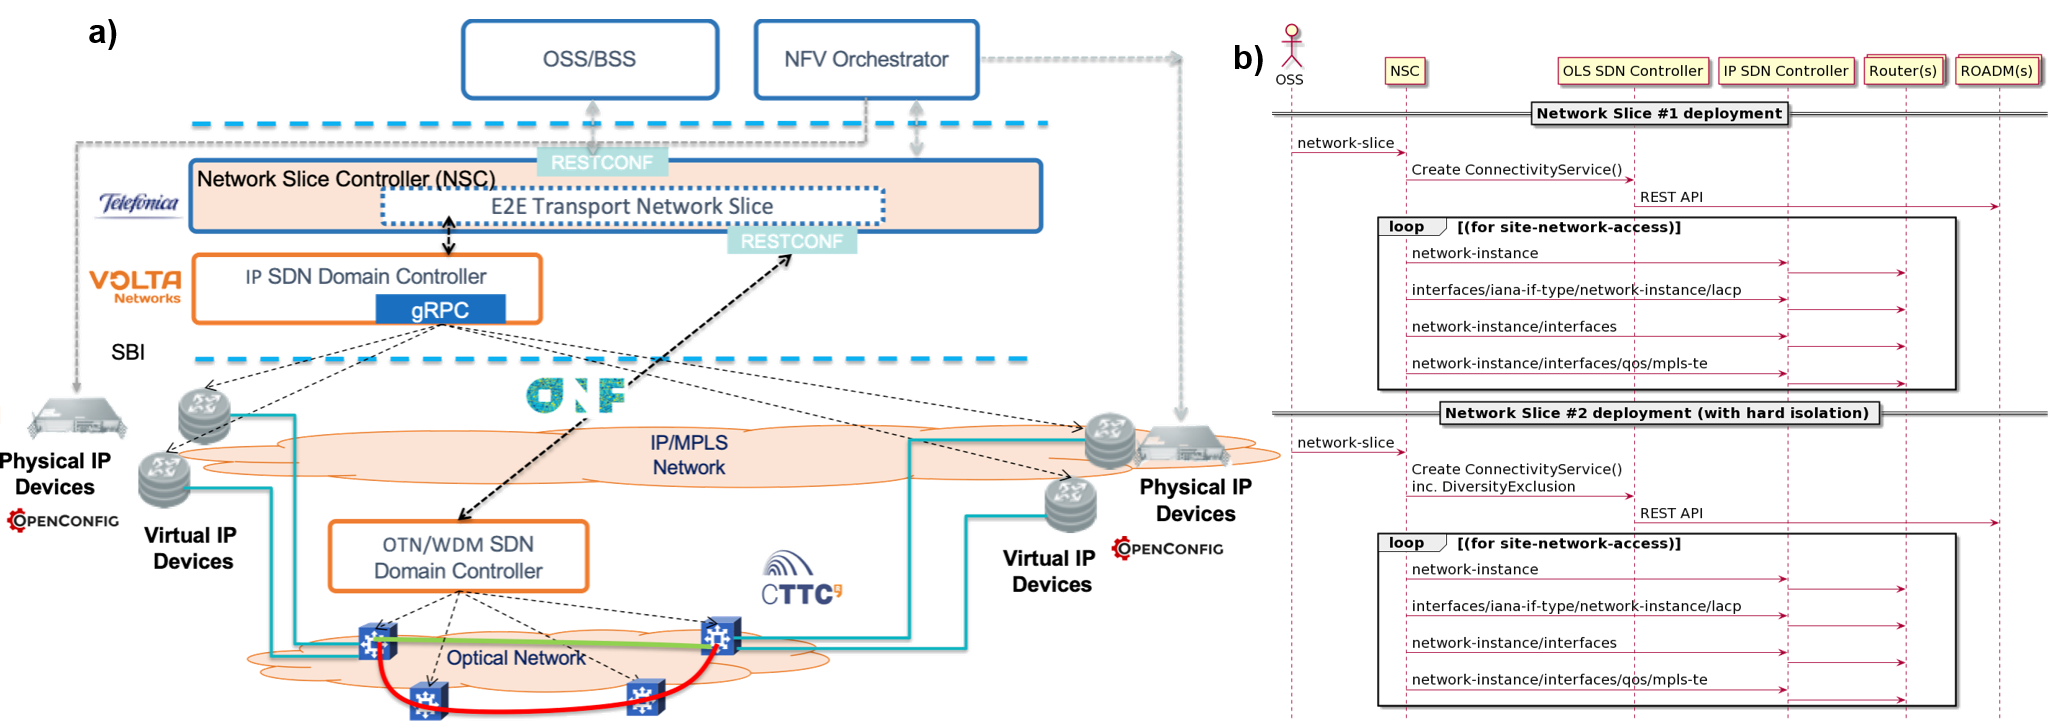
\includegraphics[width=\linewidth]{arch.png}
\vspace{-7pt} \caption{a) Overall proposed architecture; and b) Sequence diagram for multiple network slice deployment with isolation characteristics.}
\label{fig:scheme}
\vspace{-17pt}
\end{figure}

%The OSS/BSS may request that the deployed network slice is isolated from any other network slices or different services delivered to the same customers. Naturally, other network slices or services must not negatively impact the requested transport network slice's delivery. There are several possibilities to provide this isolation, which can be provided at several degrees, such as dedicated allocation of resources for a specific slice or sharing some network resources. Figure \ref{fig:results}.a shows the multiple isolation options that range from a hard slice to a soft slice: a) no-isolation, meaning that slices are not separated; b) physical-isolation, where slices are completely physically separated, for example, in different locations; c) logical-isolation, where slices are logically separated, only a certain degree of isolation is performed through QoS mechanisms; d) process-isolation, where slices include process and threads isolation; e) physical-network-isolation, where slices contain physically separated links; f) virtual-resource-isolation, where slices have dedicated virtual resources; g) network-functions-isolation, where Network Function (NF) are dedicated to a single network slice; h) service-isolation, where virtual resources and NFs are shared.

%Figure \ref{fig:scheme}.b shows the proposed workflow to deploy hard and soft transport network slices. In the workflow, two isolated network slices are deployed. The first one allocates a connectivity service to interconnect both IP layer domains (see for reference Figure \ref{fig:scheme}.a). This triggers the necessary optical configuration mechanism to each of the underlying ROADMs (e.g., using OpenROADM protocol). 

%Once the connectivity service has been established, the NSC is responsible for requesting to IP SDN domain controller the necessary virtual routers (in the proposed scenario, two site-network-access are configured, one network instance on each site). Link Aggregation Control Protocol (LACP) is configured to each network instance. Then interfaces are aggregated and properly configured using dedicated VLAN or MPLS-TE mechanisms. 

%When a new isolated slice is requested, NSC can request a dedicated and isolated connectivity service to the underlying optical SDN controller. Figure \ref{fig:results}.b details the available connectivity constraint to provide disjoint path selection using ONF Transport API. It consists of including a diversity exclusion constraint with the previous connectivity service identifier. Later, at IP layer novel virtual routers are deployed to provide the requested degree of isolation.


%%%%%%%%%%%%%%%%%%%%%%%%%%%%%%%%%%%%%%%%%%
\section{Results}


%The experimental testbed has been set-up at Telefónica (NSC deployment and Volta Elastic Virtual Routing Engine stacked in 7316 Edgecore hardware) and CTTC laboratories (including a T-API SDN controller over a flexi-grid 4-nodes DWDM network), as depicted in Figure \ref{fig:scheme}.a. In order to properly set-up transport, we have introduced the transport network slice YANG data model in the RESTCONF server of NSC. An example of requested transport network slice is depicted in Figure \ref{fig:results}.c. It can be observed that several levels of isolation can be requested per node, link and slice. 

%In order to validate the depicted sequence diagram in Figure \ref{fig:scheme}.b, we provide the captured Wireshark traces among the complete system to deploy a complete hard slice request (the figure provides the selected significant traces). In this figure the different involved protocols can be observed. Firstly it shows the request for the transport network slice. It is quickly stored and answered, as it is processed after response (later an status update might be requested). 

%The transport network slice requests physical network isolation for the solicited link, thus a T-API connectivity service is requested including as connectivity constraints the diversity exclusion option. For that, we provide the identifiers from the previous established connectivity services and we obtain a disjoint path for the new requested slice, resulting in the requested physical network isolation (Figure \ref{fig:results}.b). It can be appreciated that the connectivity service setup time is 2.001s. Consider that the ADRENALINE testbed already has the paths equalized. 

\begin{figure}[tb]%[htdp]
\centering
	\centering
		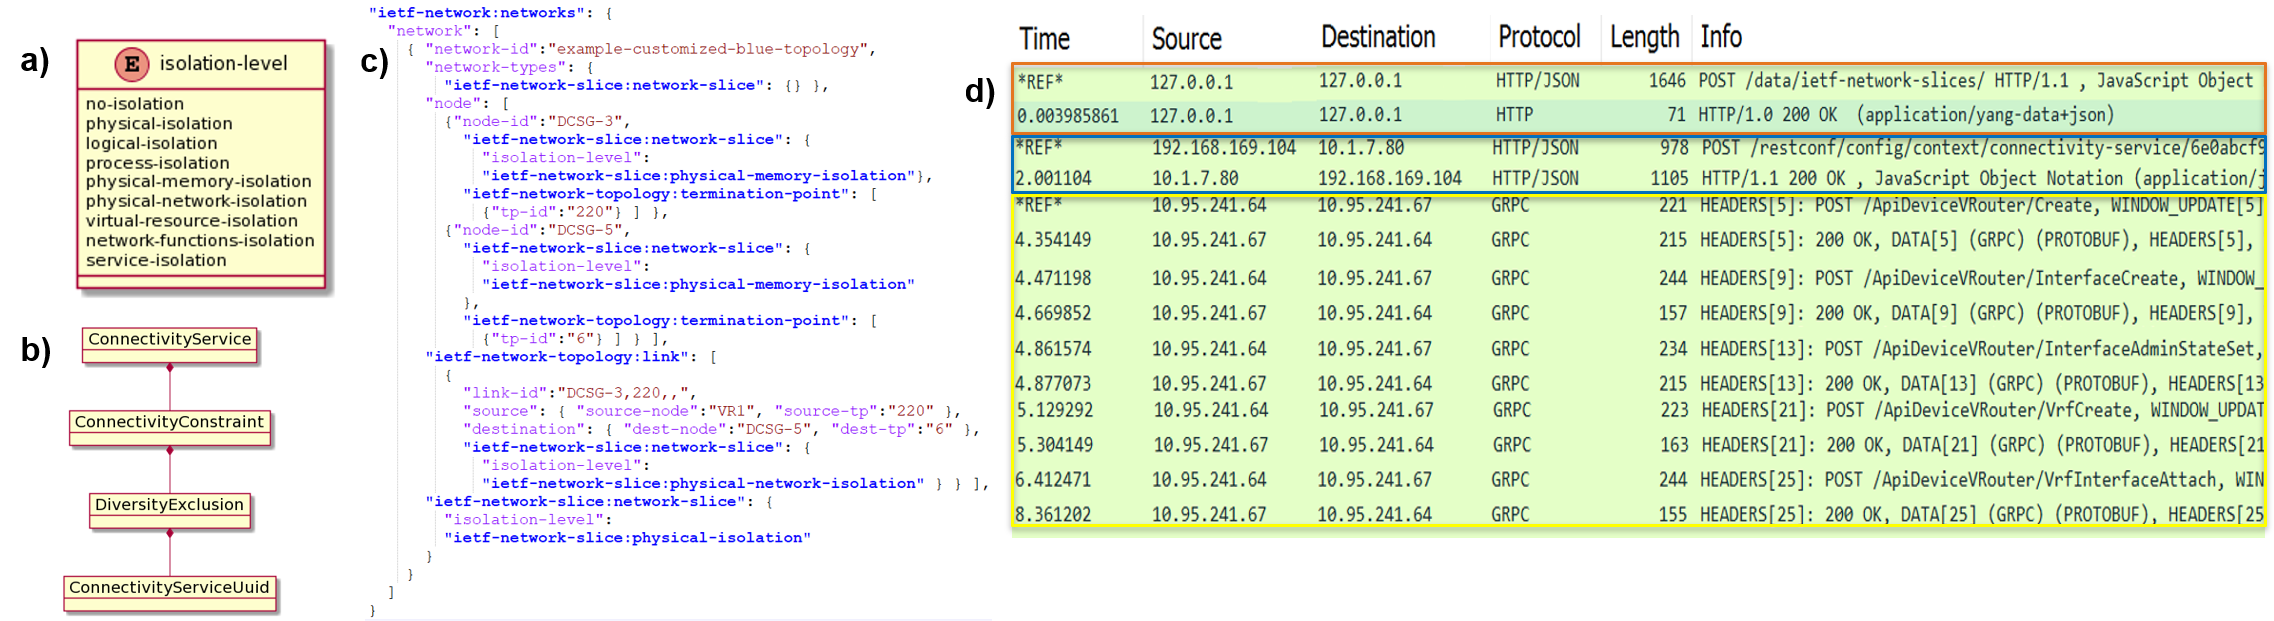
\includegraphics[width=\linewidth]{results.png}
\vspace{-7pt} \caption{a) Network Slice isolation levels; b) Disjoint path selection using ONF Transport API; c) Example of transport slice request; and d) Wireshark captures for deployment of a hard slice.}
\label{fig:results}
\vspace{-17pt}
\end{figure}


%Finally, the virtual routers (vRouter) are created and properly setup. The Wireshark capture shows the internal gRPC protocol from Volta Networks, which is equivalent to OpenConfig calls, for the vRouter deployment and configuration. It includes a call to create a new vRouter on top of Edgecore hardware. Then, interfaces are incorporated to the vRouter and configured. Later, Virtual routing and forwarding (VRF) table is setup and finally interfaces are attached to the VRF. This process set-up delay is of 8.36s. 



\section{Conclusions - Victor}

%We have presented and validated an end-to-end architecture that allows the deployment of transport network slices with several degrees of isolation. The results indicate the feasibility of deployment of multi-layer IP over DWDM transport network slices bsed on virtual roauters and optical disjoint paths to provide hard isolation. Soft isolation is instead reached through connectivity constraints and L2VPN service router configuration.

%%%%%%%%%%%%%%%%%%%%%%%%%%%%%%%%%%%%%%%%%%

%\funding{Please add: ``This research received no external funding'' or ``This research was funded by NAME OF FUNDER grant number XXX.'' and  and ``The APC was funded by XXX''. Check carefully that the details given are accurate and use the standard spelling of funding agency names at \url{https://search.crossref.org/funding}, any errors may affect your future funding.}


\acknowledgments{In this section you can acknowledge any support given which is not covered by the author contribution or funding sections. This may include administrative and technical support, or donations in kind (e.g., materials used for experiments).}


\reftitle{References}

% Please provide either the correct journal abbreviation (e.g. according to the “List of Title Word Abbreviations” http://www.issn.org/services/online-services/access-to-the-ltwa/) or the full name of the journal.
% Citations and References in Supplementary files are permitted provided that they also appear in the reference list here. 

%=====================================
% References, variant A: external bibliography
%=====================================
%\externalbibliography{yes}
%\bibliography{your_external_BibTeX_file}

%=====================================
% References, variant B: internal bibliography
%=====================================
\begin{thebibliography}{999}
% Reference 1
\bibitem{transportslice21}
R. Rokui, et al., Definition of IETF Network Slices, IETF draft draft-ietf-teas-ietf-network-slice-definition-00, 2021.

\bibitem{casellas20}
R. Casellas, et al., Virtualization of disaggregated optical networks with open data models in support of network slicing. JOCN Feb 1;12(2):A144-54, 2020.

%\bibitem{abno15}
%A. Aguado, et al., ABNO: a feasible SDN approach for multi-vendor IP and optical networks, JOCN, 2015, Vol. 7. Iss. 2.

\bibitem{tapiextensions20}
R. Vilalta, et al., Transport API extensions for the interconnection of multiple NFV infrastructure points of presence. OFC, 2019.

\bibitem{openconfig}
A. Shaikh, et al., Vendor-neutral network representations for transport SDN. OFC, 2016.


%\bibitem{yangslice}
%X. Liu, et al., IETF Network Slice YANG Data Model, IETF draft draft-liu-teas-transport-network-slice-yang-02, 2020.

\bibitem{transportslicemodel}
X. Liu, et al., IETF Network Slice YANG Data Model, IETF draft-liu-teas-transport-network-slice-yang-02, 2020.

\bibitem{ifusion}
L. Contreras, et al., FUSION: Standards-based SDN Architecture for Carrier Transport Network. CSCN, 2018.

\bibitem{restconf}
A. Bierman, M. Bjorklund, K. Watsen, R. Fernando, RESTCONF protocol. IETF RFC 8040, 2017.
\end{thebibliography}

% If authors have biography, please use the format below
%\section*{Short Biography of Authors}
%\bio
%{\raisebox{-0.35cm}{\includegraphics[width=3.5cm,height=5.3cm,clip,keepaspectratio]{Definitions/author1.pdf}}}
%{\textbf{Firstname Lastname} Biography of first author}
%
%\bio
%{\raisebox{-0.35cm}{\includegraphics[width=3.5cm,height=5.3cm,clip,keepaspectratio]{Definitions/author2.jpg}}}
%{\textbf{Firstname Lastname} Biography of second author}

% The following MDPI journals use author-date citation: Arts, Econometrics, Economies, Genealogy, Humanities, IJFS, JRFM, Laws, Religions, Risks, Social Sciences. For those journals, please follow the formatting guidelines on http://www.mdpi.com/authors/references
% To cite two works by the same author: \citeauthor{ref-journal-1a} (\citeyear{ref-journal-1a}, \citeyear{ref-journal-1b}). This produces: Whittaker (1967, 1975)
% To cite two works by the same author with specific pages: \citeauthor{ref-journal-3a} (\citeyear{ref-journal-3a}, p. 328; \citeyear{ref-journal-3b}, p.475). This produces: Wong (1999, p. 328; 2000, p. 475)

%%%%%%%%%%%%%%%%%%%%%%%%%%%%%%%%%%%%%%%%%%
%% for journal Sci
%\reviewreports{\\
%Reviewer 1 comments and authors’ response\\
%Reviewer 2 comments and authors’ response\\
%Reviewer 3 comments and authors’ response
%}
%%%%%%%%%%%%%%%%%%%%%%%%%%%%%%%%%%%%%%%%%%
\end{document}

